\documentclass[10pt,a4paper]{article}
\usepackage[margin=2.1cm]{geometry}
\usepackage{amsmath,amssymb,bm}
\usepackage{graphicx,booktabs,xcolor,enumitem,hyperref}
\hypersetup{colorlinks,linkcolor=blue!50!black,urlcolor=blue!50!black}
\newcommand{\kc}{\kappa_2}
\newcommand{\note}[1]{\par\smallskip\noindent\colorbox{gray!12}{\parbox{\dimexpr\linewidth-2\fboxsep}{\small #1}}\par\smallskip}
\newcommand{\evd}[1]{\textsf{\small[#1]}}
\newcommand{\simple}[1]{\par\noindent\textbf{In simple words:} #1\par\smallskip}
\title{TOP-Q --- Day 6 worked notes\\[2pt]\large Monte Carlo study 2: does pinning protect the phase an interferometer sees?}
\author{PH 5110 term paper --- Kotapati Kishore (EE26E016)}
\date{31 October 2026 (two days ahead of the revised plan)}
\begin{document}\sloppy\maketitle

\note{All results are \textbf{numerical simulations} \evd{Simulated}. Arrays T and D ($M=81$), centre-guide launch, device length $L=10$ coupling lengths $=5\pi/\kc$ unless stated. 2000 simulated chips per point = 1000 independent arm pairs. Units: $\sigma_\beta$ in $\kc$, $\sigma_\kappa$ dimensionless.}

\tableofcontents

%=====================================================================
\section{The question, made measurable}
%=====================================================================
An interferometer never measures an absolute phase. It measures the \textbf{difference} between two arms. So the Day-6 experiment (Fig.~\ref{fig:sch}) is: put two arrays of the \emph{same design} on one chip, give each its own random local errors, and compute
\[
\Delta\varphi=\delta\varphi_A-\delta\varphi_B ,
\]
where $\delta\varphi$ is each arm's phase error at the output (both definitions from Day 5: modal and output-guide). A chip-wide error (e.g.\ the whole wafer slightly thicker) shifts both arms equally and \textbf{cancels exactly} in $\Delta\varphi$ \evd{Derived}.

\begin{figure}[h]\centering
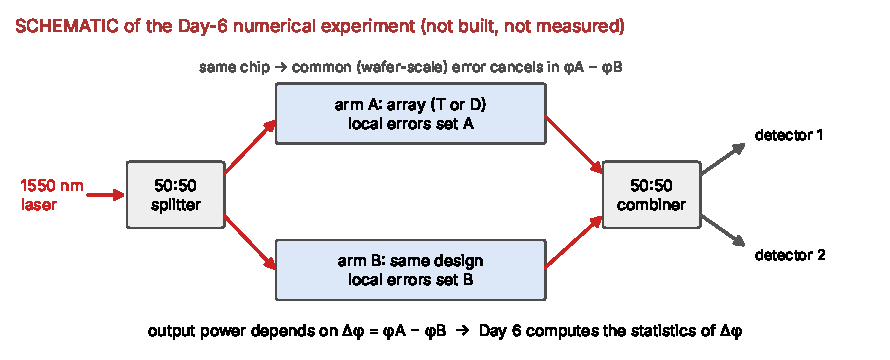
\includegraphics[width=0.85\linewidth]{../../figures/fig_two_arm_schematic.pdf}
\caption{\textbf{Schematic} of the numerical experiment (drawn by us; not built, not measured).}
\label{fig:sch}
\end{figure}

\subsection{Two numbers we report}
\begin{itemize}[itemsep=1pt]
\item \textbf{Circular standard deviation} of $\Delta\varphi$. Phases wrap around at $2\pi$, so the ordinary std is misleading for large errors. We use $R=|\langle e^{i\Delta\varphi}\rangle|$ and $\sigma_{\rm circ}=\sqrt{-2\ln R}$, which equals the ordinary std for small Gaussian errors \evd{Verified-by-test}.
\item \textbf{$R$ itself}, which has a direct meaning: if the arms of a 50:50 interferometer have a random phase difference $\Delta\varphi$, the \emph{average} fringe contrast left over is $R$ \evd{Derived: average of $\cos(\theta+\Delta\varphi)$}. $R=1$: perfect; $R=0$: no interference left on average.
\end{itemize}
First-order prediction for the modal phase: $\sigma(\Delta\varphi)\approx\sqrt2\,\cdot\,(\text{Day-3 slope})\cdot\sigma\cdot L$ (two independent arms, error grows with length).

%=====================================================================
\section{Results}
%=====================================================================
\begin{figure}[t]\centering
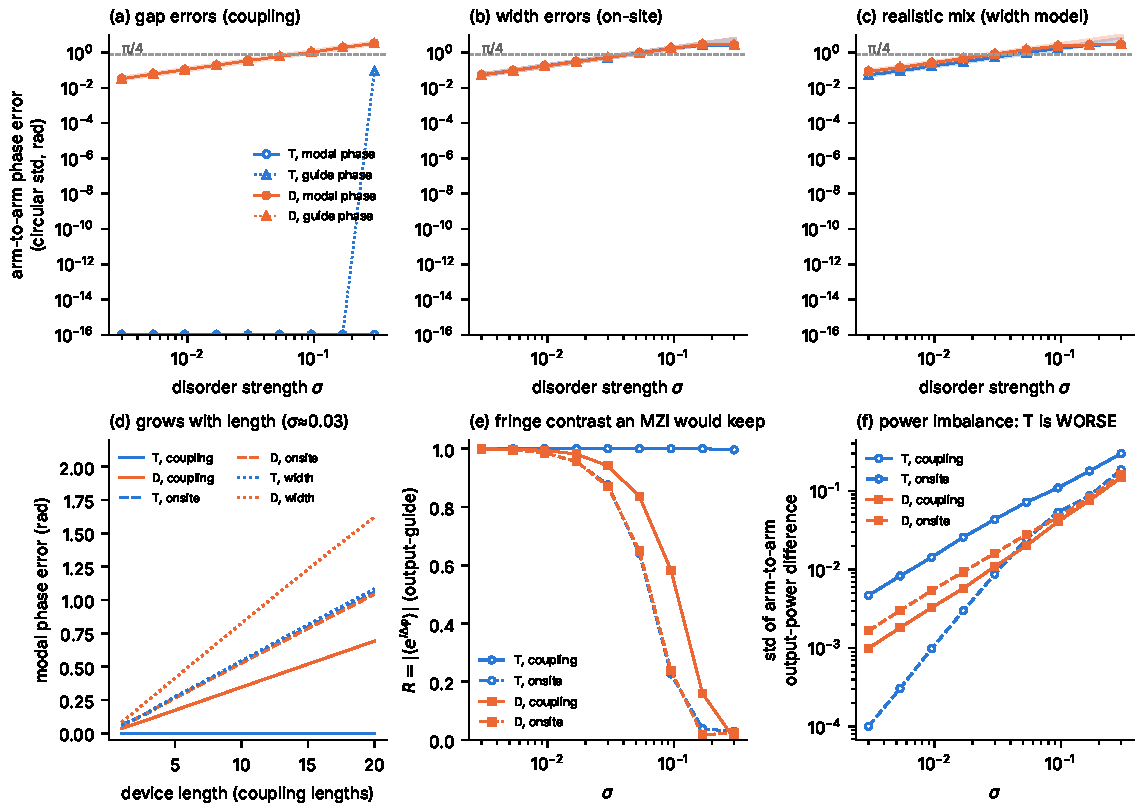
\includegraphics[width=\linewidth]{../../figures/fig_mc_phase.pdf}
\caption{\textbf{Simulation}, \texttt{scripts/day6\_mc\_phase.py} $\to$ \texttt{data/day6\_mc\_phase.npz}. (a)--(c) Arm-to-arm phase error vs.\ disorder strength (circles/squares: modal phase; triangles: output-guide phase; thick faint lines: first-order prediction). (d) Growth with device length at $\sigma\approx0.03$. (e) Fringe contrast $R$ an interferometer would keep. (f) Spread of the arm-to-arm \emph{power} difference at the output.}
\label{fig:mc}
\end{figure}

\subsection{Gap errors (chiral): phase protected}
T: $\Delta\varphi=0$ \emph{exactly} (both definitions) for every $\sigma_\kappa$ up to 0.17; at $\sigma_\kappa=0.3$ the output-guide phase flips to $\pi$ in 0.2\% of arm pairs (the Day-5 sign flip when the zero-mode weight falls below 1/2), giving $\sigma_{\rm circ}=0.09$~rad and $R=0.996$. D: $\sigma_{\rm circ}=0.35$~rad at $\sigma_\kappa=0.03$ and 1.04~rad at 0.095, matching first order ($0.34$, $1.07$). Contrast at $\sigma_\kappa=0.095$: \textbf{T 1.00, D 0.58}. \evd{Simulated}

\subsection{Width errors (not chiral): no protection}
T and D are the same within statistics: $\sigma_{\rm circ}$ = 0.17 / 0.17~rad at $\sigma_\beta=0.0095$; 0.53 / 0.53 at 0.03; contrast at 0.095: 0.23 / 0.24. First order predicts 0.171 and 0.540 for both. \evd{Simulated}

\subsection{Realistic mix (width model, $\sigma_\beta=\sigma_\kappa$)}
T's phase error is about 0.66 of D's (0.54 vs 0.83 rad at $\sigma=0.03$), exactly the Day-4 eigenvalue ratio: the phase inherits it through $\delta\varphi\approx\delta b\,L$. As on Day 4, this ratio depends on the unknown $\sigma_\beta/\sigma_\kappa$ of real waveguides.

\subsection{Length: errors grow in proportion}
Fig.~\ref{fig:mc}d: every unprotected phase error grows linearly with $L$; T under gap errors stays at 0 for all lengths up to 20 coupling lengths.

\subsection{A tolerance number}
Requiring $\sigma_{\rm circ}<\pi/4$ at 10 coupling lengths (a loose target) allows on-site disorder only up to about $\sigma_\beta\approx0.045\,\kc$ \emph{for both arrays}. In words: the random spread of each guide's propagation constant must be below about 5\% of the strong coupling. Converting this to nanometres of width needs $\partial\beta/\partial w$ (mode solver; open question Q-ratio).

\subsection{The surprise: T has MORE power imbalance under gap errors}
Fig.~\ref{fig:mc}f. Spread of the arm-to-arm difference in output power:\par\smallskip\noindent
\begin{tabular}{@{}lcccc@{}}\toprule
 & T, gap errors & D, gap errors & T, width errors & D, width errors\\\midrule
$\sigma=0.003$ & 0.005 & 0.001 & 0.0001 & 0.002\\
$\sigma=0.03$ & 0.043 & 0.011 & 0.009 & 0.016\\\bottomrule
\end{tabular}
\smallskip

Under gap errors, T's output power varies \textbf{4--5$\times$ more} than D's, and it grows in proportion to $\sigma$ (first order). Reason \evd{Derived (qualitative)}: the pinned zero mode keeps $b=0$ but its \emph{shape} changes (Day 4), so its weight $w_0$ on the input/output guide changes in proportion to the coupling error; the output power $\approx w_0^2+\dots$ follows. Under width errors, T's power changes only at second order (its phase moves, its shape barely does).
\note{\textbf{The pattern across Days 4--6.} Topological protection \emph{moves} gap errors from the phase into the amplitude: it does not remove them. Loss behaves the same way (Day 5). For an interferometer, an amplitude imbalance between arms also lowers the contrast --- Days 8--10 will put both effects into one number.}

%=====================================================================
\section{What Day 6 answers}
%=====================================================================
\begin{tabular}{@{}p{0.27\linewidth}p{0.66\linewidth}@{}}\toprule
Question & Answer (simulation, this model)\\\midrule
Does pinning protect the arm-to-arm phase? & \textbf{Yes, exactly, for gap (coupling) errors} --- both phase definitions --- until the zero mode loses half its weight on the port (rare below $\sigma_\kappa\approx0.3$).\\
For width errors? & \textbf{No.} Identical to an ordinary defect of the same confinement.\\
For a real mix? & Partly; the benefit depends on $\sigma_\beta/\sigma_\kappa$ (unknown).\\
For free? & \textbf{No.} Under gap errors T's output power varies more than D's.\\
Chip-wide errors? & Cancel in any two-arm device, topological or not.\\\bottomrule
\end{tabular}

%=====================================================================
\section{Hardware: how arm-to-arm phase errors are measured on real chips}
%=====================================================================
\textbf{Not done by us.} The images in our chat (from published papers) show the standard methods:
\begin{itemize}[itemsep=1pt]
\item \textbf{Unbalanced on-chip MZIs:} the two arms have different lengths, so the transmission spectrum shows fringes vs.\ wavelength; a phase error shifts the fringes sideways, and the shift is read off directly.
\item \textbf{Wafer-scale automatic testing:} many nominally identical MZIs across a wafer are measured by a probe station; histograms of the measured phase error, imbalance and insertion loss are the real-world version of our Monte Carlo distributions.
\end{itemize}
These are exactly the data that would test our predictions --- and the data that would fix $\sigma_\beta$ and $\sigma_\kappa$ for a real process. Cite the source papers shown with each image before reusing them.

\section{Code and tests}
New in \texttt{topq/montecarlo.py}: \texttt{run\_propagation\_ensemble} (all lengths from one diagonalisation), \texttt{clean\_amplitudes}, \texttt{phase\_stats} (circular statistics). Scripts: \texttt{day6\_mc\_phase.py} (84~s), \texttt{day6\_two\_arm\_schematic.py}. 3 new tests (agreement with direct propagation to $10^{-12}$; T differential phase exactly zero under coupling disorder; circular-statistics limits). Suite: \textbf{96 passed}.

\section{Self-test}
\begin{enumerate}[itemsep=1pt]
\item Why does a chip-wide thickness error not appear in $\Delta\varphi$?
\item Why use the circular std instead of the ordinary std?
\item Show that the average fringe contrast left is $R=|\langle e^{i\Delta\varphi}\rangle|$.
\item Why does the phase error grow linearly with length?
\item Why does T's output \emph{power} vary more than D's under gap errors, even though its phase does not?
\item What one measurement on a real wafer would tell you whether TOP-Q's protection is useful?
\end{enumerate}
\end{document}
